\subsection*{Phần 1: Giới thiệu Toán học}
\noindent\textbf{1.} Để chứng minh công thức \eqref{eq:p31} ta cần sử dụng các phép xấp xỉ cho hàm mũ:
\begin{equation}
  \label{eq:31}
  \sqrt{a^{2} + x^{2}} = a \left( 1 + \frac{x^{2}}{a^{2}} \right)^{1/2} \approx a \left( 1 + \frac{x^{2}}{2a^{2}} \right) = a + \frac{x^{2}}{2a}
\end{equation}

\noindent\textbf{2.} Phương trình của đường tròn được mô tả có dạng:
\begin{equation}
  \label{eq:32}
  x^{2} + (y - R)^{2} = R^{2}
\end{equation}
sử dụng công thức \eqref{eq:p31} trong đề bài ta được:
\begin{equation}
  \label{eq:33}
  x^{2} + (y - R)^{2} = R^{2} \implies y - R = \pm \sqrt{R^{2} - x^{2}} \implies y = R - \frac{x^{2}}{2R}
\end{equation}

\subsection*{Phần 2: Sự đẳng thời}
\begin{wrapfigure}[11]{r}{6cm}
  \centering
  \vspace{-4mm}
  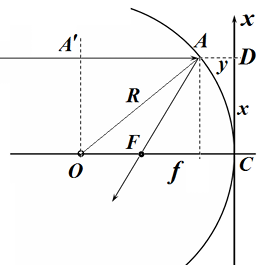
\includegraphics[width=0.3\textwidth]{Figures/P3/Fig 3.1S.png}
\end{wrapfigure}

\noindent\textbf{1.} Ta có thể xem tiêu điểm là ảnh của một điểm sáng nằm tại vô cùng. Theo nguyên lý đẳng thời cho sự  tạo ảnh, ta cần chứng minh rằng tồn tại một điểm $F$ mà  thời gian ánh sáng chuyển động đến $F$ là như nhau với mọi tia sáng. Do tính đối xứng, điểm này phải nằm trên quang trục. Trong trường hợp này ánh sáng truyền đi trong môi trường đồng nhất, nên để thời gian truyền là bằng nhau, chiều dài các đường truyền phải bằng nhau. Lấy một tia bất kỳ $AA' $ song song với quang trục , cách quang trục một đoạn $x=CD$. Vì các tia tới là song song, khoảng cách từ điểm vật ở vô cùng đến bất kỳ mặt phẳng nào vuông góc với các tia (và trục quang học chính) là như nhau. Để đơn giản, chọn mặt phẳng $A'O $, đi qua tâm hình học của gương. Khi đó, điều kiện đẳng thời có thể được phát biểu như sau: phải tồn tại một điểm $F$ sao cho khoảng cách $ AF + A'F = l $ không phụ thuộc vào $ x $. Từ hình vẽ, khoảng cách này được biểu diễn qua các tham số của hệ dưới dạng:
\begin{equation}
  \label{eq:34}
  l = f + \sqrt{(R - y)^{2} + x^{2}} = (R - y) + \sqrt{f^{2} + x^{2}}
\end{equation}
trong đó $ y = AD $; $ f = CF $ là tiêu cự của gương (nếu tiêu điểm tồn tại). Bây giờ, ta cần tìm một hàm $ y = f(x) $ sao cho biểu thức trên luôn thỏa mãn với mọi $ x $. Thực hiện các biến đổi đại số đơn giản, ta có:
\begin{equation}
  \label{eq:35}
  \sqrt{x^{2} + (f-y)^{2} } = y + f \implies x^{2}+f^{2}-2yf+y^{2}=y^{2}+2yf+f^{2}\implies 4yf=x^{2}
\end{equation}
tức bề mặt của gương là một đường parabol:
\begin{equation}
  \label{eq:36}
  y = \frac{x^{2}}{4f}
\end{equation}
thì tất cả các tia song song với trục quang học sẽ đến điểm $ F $ cùng một lúc, do đó điểm này sẽ là tiêu điểm.
Nói cách khác, nếu gương có dạng parabol, các tia luôn hội tụ tại $F$. Như đã chỉ ra, đối với các tia bàng trục, cung tròn có thể xem như một đoạn parabol, hay có thể phát biểu ngược lại: parabol có thể được thay thế bằng cung tròn. Ta có:
\begin{equation}
  \label{eq:37}
  y = \frac{x^{2}}{2R} \quad \text{thì} \quad f = \frac{R}{2}
\end{equation}
tiêu cự gương cầu:
\begin{equation}
  \label{eq:38}
  f = \frac{R}{2}
\end{equation}

\begin{wrapfigure}[11]{r}{8cm}
  \centering
  \vspace{-4mm}
  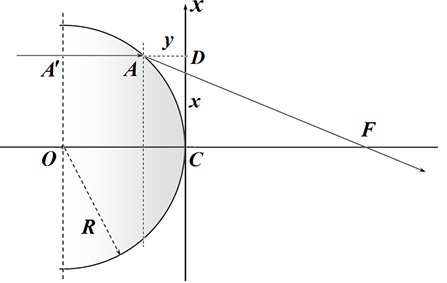
\includegraphics[width=0.45\textwidth]{Figures/P3/Fig 3.2S.png}
\end{wrapfigure}

\noindent\textbf{2.} Lập luận tương tự ý trước điều kiện tồn tại của tiêu điểm là: thời gian mà ánh sáng đi qua khoảng cách $AF + A'A$ không phụ thuộc vào khoảng cách $x$ từ tia sáng đến quang trục. Giả sử ánh sáng truyền đi một khoảng cách $ l $ trong môi trường đồng nhất có chiết suất $ n $, khi đó thời gian truyền bằng:
\begin{equation}
  \label{eq:39}
  t = \frac{l}{c/n} = \frac{nl}{c}
\end{equation}
với $c/n $ là tốc độ ánh sáng trong môi trường này. Lưu ý rằng thay vì tính toán sự thay đổi của tốc độ ánh sáng (điều thực sự xảy ra), khi tính toán thời gian truyền, ta có thể coi tốc độ ánh sáng không đổi (và bằng tốc độ ánh sáng trong chân không $ c $) nhưng độ dài đường truyền tăng lên thành $ nl $ (trong quang học, đại lượng này được gọi là độ dài đường đi quang học). Do đó, điều kiện tồn tại của tiêu điểm là đẳng thức sau được thỏa mãn với mọi giá trị của $ x $:
\begin{equation}
  \label{eq:310}
  n(R-y)+\sqrt{x^{2}+(f+y)^{2}}=nR+f
\end{equation}
biến đổi ta được:
\begin{equation}
  \label{eq:311}
  \sqrt{x^{2}+(f+y)^{2}}=f+ny\implies x^{2}+f^{2}+2fy+y^{2}=f^{2}+2fny+n^{2}y^{2}\implies x^{2}=2(n-1)fy
\end{equation}
nếu mặt cong của thấu kính được mô tả bằng phương trình:
\begin{equation}
  \label{eq:312}
  y = \frac{x^{2}}{2(n - 1)f}
\end{equation}
thì đẳng thức \eqref{eq:310} sẽ được thỏa mãn với mọi giá trị của $ x $, tức $ F $ là tiêu điểm. Nhưng hàm này mô tả trong xấp xỉ paraxial một "cung tròn" có bán kính $ R $:
\begin{equation}
  \label{eq:313}
  y = \frac{x^{2}}{2R}
\end{equation}
do đó, thấu kính được mô tả trong điều kiện bài toán có tiêu điểm. Để xác định tiêu cự của thấu kính, ta chỉ cần so sánh các biểu thức \eqref{eq:312} và \eqref{eq:313}, từ đó suy ra rằng tiêu cự này bằng:
\begin{equation}
  \label{eq:314}
  f = \frac{R}{n-1}
\end{equation}

\begin{wrapfigure}[10]{r}{8cm}
  \centering
  \vspace{-8mm}
  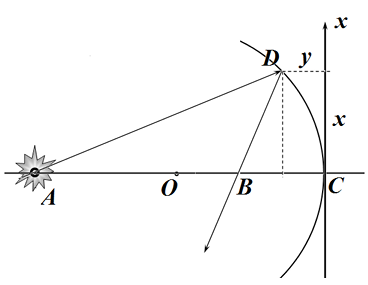
\includegraphics[width=0.4\textwidth]{Figures/P3/Fig 3.3S.png}
\end{wrapfigure}

\noindent\textbf{3a.} Tương tự như các bài toán trước: để tồn tại ảnh tại điểm $B$, khoảng cách $ DB + AD $ không phụ thuộc vào vị trí của điểm $ D $ trên bề mặt gương và bằng khoảng cách $ CB + AC $. Điều kiện này sẽ được thỏa mãn nếu đẳng thức:
\begin{equation}
  \label{eq:315}
  \sqrt{x^{2}+(a-y)^{2}}+\sqrt{x^{2}+(b-y)^{2}}=a+b
\end{equation}
được thỏa mãn với mọi $ x $. Bình phương tổng của các căn thức là một bài toán không đơn giản, vì vậy chúng ta sẽ sử dụng các công thức gần đúng để biến đổi đẳng thức \eqref{eq:315}. Trước tiên, ta sẽ viết lại \eqref{eq:315} dưới dạng:
\begin{equation}
  \label{eq:316}
  \sqrt{x^{2}+(a-y)^{2}}+\sqrt{x^{2}+(b-y)^{2}}\approx \sqrt{x^{2}+a^{2}-2ay}+\sqrt{x^{2}+b^{2}-2by}
\end{equation}
ở đây, ta đã bỏ qua các số hạng $ y^{2} $, nhưng giữ lại các số hạng $ x^{2} $. Trước đó, ta đã chỉ ra rằng đối với đường tròn (và tiếp tuyến parabol), đại lượng $ y $ tỷ lệ với $ x^{2} $, vì vậy các đại lượng này là các số hạng nhỏ cùng bậc. Đại lượng $ y^{2} $ tỷ lệ với $ x^{4} $, do đó có thể bỏ qua nó. Sử dụng mối quan hệ giữa các đại lượng nhỏ này, chúng ta tiếp tục các biến đổi đại số, sử dụng công thức \eqref{eq:p31} được cho trong đề bài:
\begin{equation}
  \label{eq:317}
  \sqrt{x^{2}+a^{2}-2ay}+\sqrt{x^{2}+b^[2]-2by}\approx a+\frac{(x^{2}-2ay)}{2a}+b+\frac{(x^{2}-2by)}{2a}
\end{equation}
thay vào \eqref{eq:315}:
\begin{equation}
  \label{eq:318}
  a+\frac{(x^{2}-2ay)}{2a}+b+\frac{(x^{2}-2by)}{2a}=a+b
\end{equation}
từ đó suy ra rằng \eqref{eq:315} sẽ được thỏa mãn với nếu hàm $ y(x) $ có dạng như sau:
\begin{equation}
  \label{eq:319}
  y=\frac{x^{2}}{4a}+\frac{x^{2}}{4b}=\left(\frac{1}{a}+\frac{1}{b}\right)\frac{x^{2}}{4}
\end{equation}
một lần nữa, chúng ta nhận được phương trình của parabol, có thể coi như parabol tiếp tuyến với đường tròn. So sánh biểu thức \eqref{eq:319} với phương trình "parabol" của đường tròn:
\begin{equation*}
  y = \frac{x^{2}}{2R}
\end{equation*}
ta có thể nhận thấy rằng tồn tại một giá trị $ b $, mà đẳng thức (15) được thỏa mãn với mọi tia sáng phát ra từ điểm $ A $. Nghĩa là ảnh của điểm này tồn tại.\\

\noindent\textbf{3b.} Từ \eqref{eq:319} và phương trình "đường tròn", ta có công thức gương cần tìm:
\begin{equation}
  \frac{1}{a}+\frac{1}{b}=\frac{2}{R}=\frac{1}{f}
\end{equation}
ở đây, ta đã sử dụng giá trị tiêu cự đã nhận được trước đó $ f = \dfrac{R}{2} $.\\

\noindent\textbf{4a.} Trong trường hợp này, các tia sáng xuất phát từ điểm $A$ và phản xạ từ gương sẽ không giao nhau. Nhưng chúng có thể giao nhau tại một điểm kéo dài của các tia phản xạ. Giả sử rằng để kéo dài các tia, khoảng cách phải được coi là âm. \\

\begin{wrapfigure}[10]{r}{8cm}
  \centering
  \vspace{-8mm}
  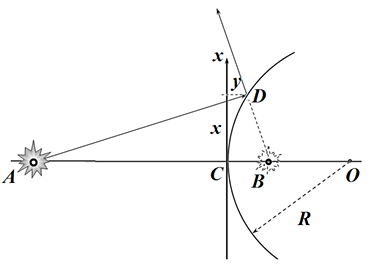
\includegraphics[width=0.42\textwidth]{Figures/P3/Fig 3.4S.png}
\end{wrapfigure}

\noindent\textbf{4b.} Trong khuôn khổ giả định này, điều kiện tồn tại của ảnh ảo được phát biểu như sau: khoảng cách $DB-AD$ là như nhau đối với tất cả các tia phản xạ từ gương, và bằng $CB-AC=b-a$. Điều kiện này được viết dưới dạng đẳng thức, tương tự như (15):
\setcounter{equation}{19}
\begin{equation}
  \label{eq:320}
  \sqrt{x^{2}+(a+y)^{2}}-\sqrt{x^{2}+(b-y)^{2}}=a-b
\end{equation}
biến đổi ta được:
\begin{align}
  \label{eq:321}
   & \sqrt{x^{2}+(a+y)^{2}}-\sqrt{x^{2}+(b-y)^{2}}\approx\sqrt{x^{2}+a^{2}+2ay}-\sqrt{x^{2}+b^{2}-2by}                                 \\
   & \approx \left(a+\frac{x^{2}+2ay}{2a}\right)-\left(b+\frac{x^{2}-2by}{2b}\right)=a-b\implies\frac{x^{2}}{2a}-\frac{x^{2}}{ab}+2y=0
\end{align}
sử dụng "phương trình parabol" của đường tròn:
\begin{equation*}
  y=\frac{x^{2}}{2R}
\end{equation*}
ta có:
\begin{equation}
  \label{eq:322}
  \frac{1}{a}-\frac{1}{b}=-\frac{2}{R}
\end{equation}
công thức này tương tự với "công thức gương cầu lõm" nếu:
\begin{itemize}
  \item Khoảng cách đến ảnh ảo là âm;
  \item Tiêu cự cũng phải là âm $f=-\frac{R}{2}$.
\end{itemize}

\noindent\textbf{4c.} Quang học hình học là một xấp xỉ của quang học sóng. Do đó, nguyên lý đẳng thời có thể được giải thích như sau:
\begin{itemize}
  \item Mỗi tia sáng có thể tương ứng với một sóng nào đó;
  \item  Nếu tất cả các sóng này đi từ nguồn đến ảnh trong cùng một thời gian, thì các pha của chúng là giống nhau;
  \item  Kết quả là tại điểm ảnh sẽ xảy ra sự giao thoa với cường độ tối đa.
\end{itemize}

\subsection*{Phần 3: Nguyên lý Fermat}
\begin{wrapfigure}[6]{r}{8cm}
  \centering
  \vspace{-12mm}
  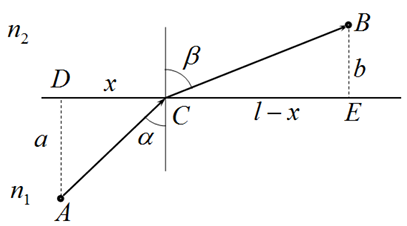
\includegraphics[width=0.4\textwidth]{Figures/P3/Fig 3.5S.png}
\end{wrapfigure}

\noindent\textbf{1.} Giả sử tia sáng đi từ điểm $A$ đến điểm $B$ (xem hình), khúc xạ tại ranh giới giữa hai môi trường tại điểm $C$. Vị trí của điểm này được xác định bởi khoảng cách $x$ tính từ điểm $D$. Đặt $DE=l$, khi đó $CE=l-x$. Thời gian di chuyển của ánh sáng theo đường $ACB$ bằng:
\begin{equation}
  \label{eq:323}
  \tau(x)=\frac{\sqrt{a^{2}+x^{2}}}{c/n_{1}}+\frac{\sqrt{b^{2}+(l-x)^{2}}}{c/n_{2}}=\frac{n_{1}\sqrt{a^{2}+x^{2}}+n_{2}\sqrt{b^{2}+(l-x)^{2}}}{c}
\end{equation}
theo nguyên lý Fermat, khi di chuyển theo quỹ đạo thực, thời gian này là nhỏ nhất, tức ta phải tìm cực trị của hàm \eqref{eq:323}
\begin{equation}
  \label{eq:324}
  \tau'(x)=\frac{2n_{1}x}{2\sqrt{a^{2}+x^{2}}}-\frac{2n_{2}(l-x)}{2\sqrt{b^{2}+(l-x)^{2}}}=0
\end{equation}
từ hình vẽ, ta có:
\begin{equation}
  \label{eq:325}
  \sin{\alpha}=\frac{x}{\sqrt{a^{2}+x^{2}}}, \quad \sin{\beta}=\frac{l-x}{\sqrt{b^{2}+(l-x)^{2}}}
\end{equation}
do đó, từ \eqref{eq:324} và \eqref{eq:325}, suy ra định luật khúc xạ ánh sáng:
\begin{equation}
  \label{eq:326}
  n_{1}\sin{\alpha}=n_{2}\sin{\beta}
\end{equation}

\begin{wrapfigure}[5]{r}{5.5cm}
  \centering
  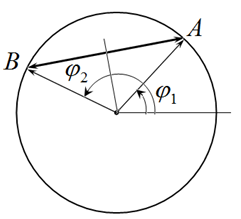
\includegraphics[width=0.25\textwidth]{Figures/P3/Fig 3.6S.png}
\end{wrapfigure}

\noindent\textbf{2a.} Để tính độ dài của quỹ đạo, ta sẽ sử dụng công thức đơn giản cho độ dài dây cung $l$ của $AB$, được viết tổng quát như sau:
\begin{equation}
  \label{eq:327}
  l=2R\lvert\sin\frac{\varphi_{1}-\varphi_{2}}{2}\rvert
\end{equation}
\begin{figure}[h]
  \centering
  \vspace{1cm}
  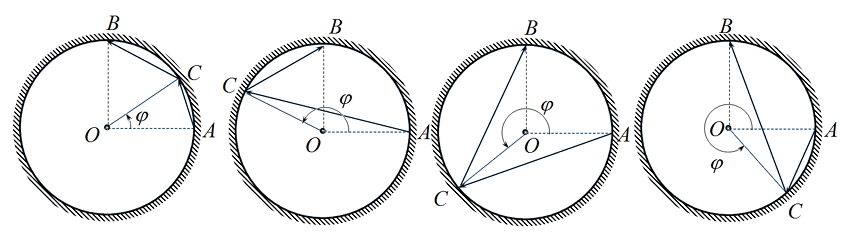
\includegraphics[width=1\textwidth]{Figures/P3/Fig 3.7S.png}
\end{figure}

\noindent độ dài quỹ đạo tia sáng với một lần phản xạ từ bề mặt trong $ACB$ bằng tổng độ dài của hai dây cung, do đó có thể được mô tả bằng công thức:
\begin{equation}
  \label{eq:328}
  L=2R\left(\sin\frac{\varphi}{2}+\lvert\sin\left(\frac{\varphi}{2}-\frac{\pi}{4}\right)\rvert\right)
\end{equation}
viết lại công thức này cho hai khoảng giá trị của góc $\phi$, khi $\phi \leqslant \dfrac{\pi}{2}$:
\begin{equation}
  \label{eq:329}
  L=2R\sin\frac{\varphi}{2}+2R\sin\frac{\pi/2-\varphi}{2}=4R\sin\frac{\pi}{8}\cos\left(\frac{\pi}{8}-\frac{\varphi}{2}\right)
\end{equation}
khi $\varphi\geqslant\dfrac{\pi}{2}$:
\begin{equation}
  \label{eq:330}
  L=2R\sin\frac{\varphi}{2}+2R\sin\frac{\varphi-\pi/2}{2}=4R\sin\left(\frac{\varphi}{2}-\frac{\pi}{8}\right)\cos\left(\frac{\pi}{8}\right)
\end{equation}

\noindent Đồ thị biểu diễn sự phụ thuộc này được chỉ ra trên hình:
\begin{figure}[h]
  \centering
  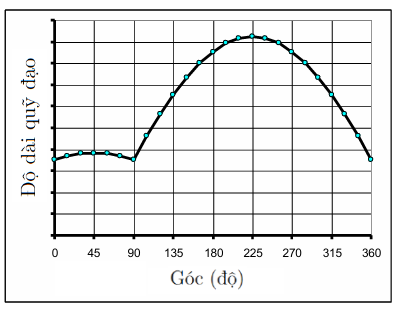
\includegraphics[width=0.6\textwidth]{Figures/P3/Fig 3.8S.png}
\end{figure}

\noindent\textbf{2b.} Các quỹ đạo thực của tia sáng thỏa mãn định luật phản xạ ánh sáng xảy ra khi:
\begin{equation}
  \label{eq:331}
  \varphi=\begin{cases}
    \dfrac{\pi}{4} \\
    \dfrac{\pi}{4}+\pi=\dfrac{5\pi}{4}
  \end{cases}
\end{equation}
với các giá trị này, độ dài của quỹ đạo là tối đa.\\

\noindent\textbf{3a.} Nguyên lý Fermat có thể được hiểu như sau: ánh sáng chọn từ nhiều con đường giữa hai điểm ra một con đường đòi hỏi thời gian cực trị (tối thiểu hoặc tối đa) hoặc thời gian tĩnh (không phụ thuộc vào quỹ đạo). Về mặt toán học, nguyên lý này được phát biểu như sau: Giả sử chiều dài của quỹ đạo được mô tả bởi một hàm số của tham số $\xi$, xác định quỹ đạo, $L(\xi)$. Khi đó, các quỹ đạo thực tương ứng với các giá trị tham số $\xi^*$, mà tại đó đạo hàm của hàm số bằng không:
\begin{equation}
  \label{eq:332}
  L'(\xi^*)=0
\end{equation}

\noindent\textbf{3b.} Giải thích nguyên lý Fermat xuất phát từ tính chất sóng của ánh sáng. Trong phạm vi lân cận điểm cực trị, khi tham số thay đổi từ giá trị tĩnh $\xi^*$ một lượng nhỏ $\Delta\xi$, chiều dài của quỹ đạo sẽ thay đổi một lượng tỉ lệ với $(\Delta\xi)^2$. Do đó, gần điểm cực trị có một phạm vi rộng của các quỹ đạo mà chiều dài của chúng thay đổi một lượng rất nhỏ. Các sóng lan truyền dọc theo những quỹ đạo này đến điểm quan sát với độ lệch pha, do đó thỏa mãn điều kiện cực đại của giao thoa.






















